\section{Semaphore}

\begin{frame}{Semaphore}
\begin{columns}
\begin{column}{0.5\textwidth}
\includegraphics[height=0.5\textheight,angle=-90]{BhfEpfenhofen_Ausfahrsignale_Talaufwaerts_II.JPG}

{\tiny \copyright 
\url{upload.wikimedia.org/wikipedia/commons/0/0b/BhfEpfenhofen\_Ausfahrsignale\_Talaufwaerts\_II.JPG}}
\end{column}
\begin{column}{0.5\textwidth}
 \begin{itemize}
  \item \cod{down}: Signal zu
  \begin{itemize}
   \item warten
  \end{itemize}
  \item \cod{up}: Signal offen
  \begin{itemize}
   \item fahren
  \end{itemize}
 \end{itemize}
\end{column}
\end{columns}
\end{frame}

\begin{frame}{Tasklet-Semaphore}
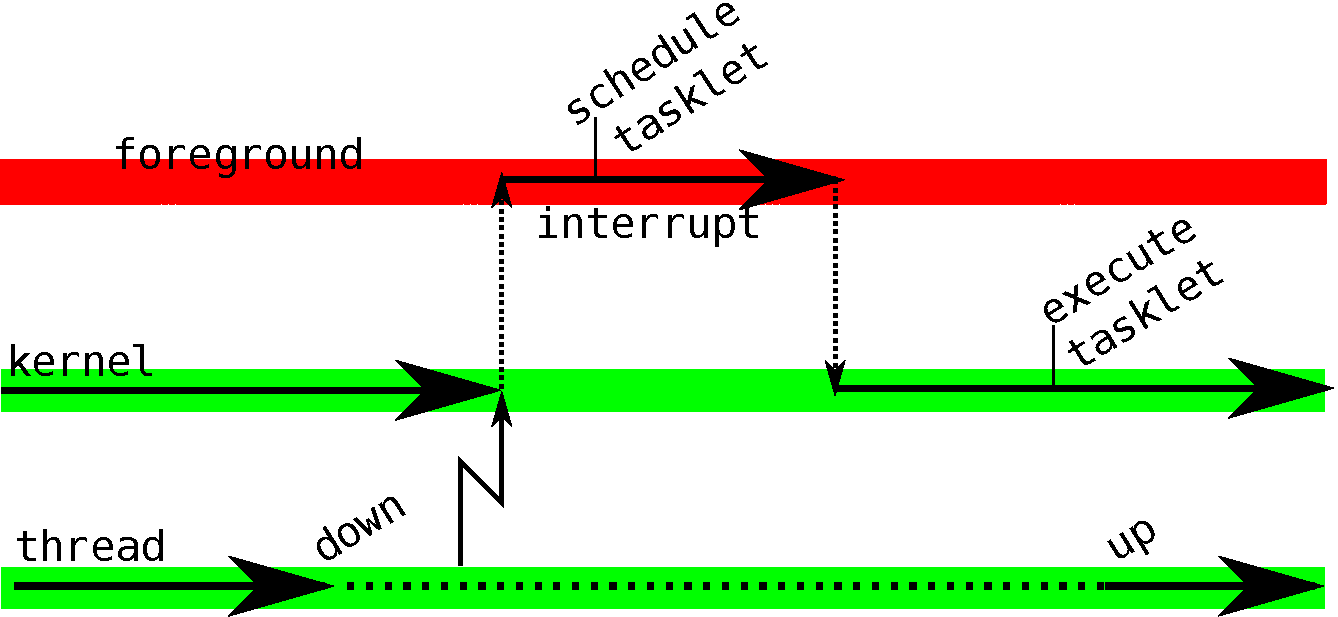
\includegraphics[width=10cm]{tasklet-semaphore.pdf}
\end{frame}

\subsection{gpio-4.c}

\begin{frame}{gpio-4.c}{schrittweise}
 \begin{itemize}
  \item Definition global 
     \href{https://elixir.bootlin.com/linux/latest/source/include/linux/semaphore.h\#L16}
          {\cod{semaphore}}
  \item Initialisation
  
   \href{https://elixir.bootlin.com/linux/latest/source/include/linux/semaphore.h\#L32}
        {\cod{sema\_init}} anfangs geschlossen 
  \item Im Tasklet
   \href{https://elixir.bootlin.com/linux/latest/source/include/linux/semaphore.h\#L44}
        {\cod{up}}: �ffne
  \item Im \cod{get\_swi}
   \href{https://elixir.bootlin.com/linux/latest/source/include/linux/semaphore.h\#L39}
        {\cod{down}}: warte \& schliesse
 \end{itemize}
\end{frame}


